% Add "answers" option to print the answers
\documentclass[addpoints,answers]{exam}

\usepackage[utf8]{inputenc}
\usepackage{calc}
\usepackage{listings}
\usepackage{xcolor}
\usepackage{xspace}

\definecolor{codegreen}{rgb}{0,0.6,0}
\definecolor{codegray}{rgb}{0.5,0.5,0.5}
\definecolor{codepurple}{rgb}{0.58,0,0.82}

\lstdefinestyle{Cstyle}{
    commentstyle=\color{codegreen},
    keywordstyle=\color{magenta},
    numberstyle=\tiny\color{codegray},
    stringstyle=\color{codepurple},
    basicstyle=\ttfamily\small,
    breakatwhitespace=true,         
    breaklines=true,                 
    captionpos=b,                    
    keepspaces=true,                 
    numbers=left,                    
    numbersep=5pt,                  
    showspaces=false,                
    showstringspaces=false,
    showtabs=false,                  
    tabsize=4
}

\lstset{style=Cstyle}

% \makebox[\textwidth]{Name:\enspace\hrulefill}
%  
% \vspace{5mm}
%\makebox[\textwidth]{Instructor’s name:\enspace\hrulefill}

\newcommand{\truefalse}
{		\begin{checkboxes}
			 \choice True
			 \choice False. Explanation: 
		\end{checkboxes}
		\vspace{10pt}
}

\newcommand{\answerspace}[1]
{
	\ifprintanswers
	\else
		\setlength{\mylength}{10pt}%
		%\noindent\rule{\mylength}{20pt}
		%\vspace{\fpeval{1.2*(#1)}}
		\vspace{#1\mylength}
	\fi
}
\newlength{\mylength}

\newcommand\pf[1]{\textcolor{red}{PF: #1}}
\newcommand\am[1]{\textcolor{blue}{AM: #1}}

\newcommand{\answer}[1]{\begin{solution}{#1}\end{solution}}
\newcommand{\ra}{$\rightarrow$\xspace}



%\usepackage{listings}
\usepackage{color}
\usepackage{lastpage}
\usepackage{verbatim}
\usepackage{fancyvrb}
\usepackage{graphicx}
\usepackage{float}
\usepackage{algorithm}
\usepackage{algpseudocode}

%\pagestyle{fancy}
%\fancyfoot[C]{{\thepage} of \pageref{LastPage}}
\newcommand{\includecode}[2][c]{\lstinputlisting[caption=, escapechar=, language=#1]{#2}<!---->}
\RecustomVerbatimCommand{\VerbatimInput}{VerbatimInput}{}

\renewcommand{\solutiontitle}{\noindent\textbf{Solution sketch: }}

\definecolor{SolutionColor}{rgb}{0.8,0.9,1}


\cfoot{Page \thepage\ of \pageref{LastPage}}

\rhead{Initials: \rule{20mm}{0.4pt}}



%%%%%%%%%%%%%%%%%%%%%%%%%%%%%%%%%%%%%%%%
\begin{document}
\fvset{numbers=left,numbersep=3pt}
\thispagestyle{empty}

\begin{center}
	{\LARGE CS408 Fall 2025 -- Homework 1 (85 points)\\}

	{\Large Deadline: Sep 12, Friday\\}

	\vspace{20mm}
\fbox{\fbox{\parbox{5.5in}{\centering
	\begin{itemize}
		\item The homework is open notes, open book.
		\item No AI tools allowed.
		\item No collaboration and no communication of any kind allowed.
		\item Provide complete and clear but concise answers. Justify thoroughly statements where required.
		\item Coding questions should be answered in C.
		\item Use basic blocks for all CFG exercises.
		\item Do not use gotos unless necessary.
	\end{itemize}
	}}}
\end{center}

\vspace{13mm}
\begin{center}
	\makebox[0.6\textwidth]{
		\combinedgradetable[h][questions]
	}
\end{center}
%\begin{center}\combinedgradetable[h][questions]\end{center}
\vspace{28mm}

\begin{center}
\makebox[\textwidth]{\textbf{Name (please print)}: \rule{100mm}{0.8pt} }
\end{center}

\newpage
\begin{questions}

\question Given the following program:
\VerbatimInput{hw1/q1_bfs.c}

\begin{parts}
\part[7]  List the elements of $N$ (nodes), $N_0$ (initial nodes),
    $N_f$ (final nodes), and $E$ (edges) that define the function's control-flow graph. Let the elements be the line numbers corresponding to the algorithm. 
    
    Your solution on gradescope should be in the form of this example:\\
    	$$N=\{1,2,3,4,5,6\}$$
    	$$N_0=\{1\}$$
    	$$N_f=\{6\}$$
    	$$E=\{[1,2],[2,4],[2,6],[3,2],[4,5],[4,3],[5,3]\}$$ \\
\answerspace{10}
\answer{
Let $N = \{1, 2, 3, 4, 5, 6, 7, 8, 9\}$, $N_0 = \{1\}$, and $N_f = \{9\}$. \\
The set of edges is given by 

    $$E = \{[1,2],[2,3],[2,8],[3,4],[4,2],[4,5],[5,6],[5,7],[6,7],[7,4],[8,9]\}$$
}

\part[5] Given the CFG from 1.1, list the elements of $N$, $N_0$, $N_f$, and $E$ that define the subgraph
with nodes 1, 2, and 3.
\answerspace{10}
\answer{
Let $N = \{1, 2, 3\}$, $N_0 = \{1\}$, and $N_f = \{\}$. The set of edges is given by $E = \{[1, 2], [2, 3]\}$.
}

\part[7] List three test cases that lead to different test paths. For each test case provided, list the corresponding test path and state explicitly the length of the test path. 

\answerspace{10}
\answerspace{10}
\answer{
    \paragraph{Test case 1:} 
    Input: graph = [[0]];
    start = 0;
    visited = [0];
    n = 1;
    Path is [1,2,3,4,5,7,4,2,8,9] , Len: 9
    \paragraph{Test case 2:} 
    Input: graph= [[0,1],
    [1,0]]; 
    start = 0;
    visited = [0,0];
    n = 2;
    \\
    Path is 
    [1,2,3,4,5,7,4,5,6,7,4,2,3,4,5,7,4,2,8,9] Len: 19
    \paragraph{Test case 3:} Input: graph=[[0,1,0],[1,0,1],[0,1,0]], start = 0, visited =[0,0,0], n=3;
    \\
    Path is [1,2,3,4,5,7,4,5,6,7,4,5,7,4,2,3,4,5,7,4,5,7,4,5,6,7,4,2,3,4,5,7,4,5,7,4,5,7,4,2,8,9], Len: 41
}

\end{parts}



\question Read this faulty program, which includes a test case  that results in failure.
\VerbatimInput{hw1/q2_copyarr.c}

\begin{parts}
\part[7] Identify the fault, and fix the fault.
\answerspace{10}
\answer {
    The fault is in line 7: \texttt{int mod\_2 = x\%3}. For positive even numbers, the check is done by taking modulus of the number with 3, which is a wrong way to find if a number is even.
    Fix: \texttt{int mod\_2 = x\%2}
}
\part[5] If possible, identify a test case that does not execute the fault.
\answerspace{10}
\answer {
    Test case: x = -1. If $x<0$, the function does not execute the faulty line.
}

\part[10] If possible, identify a test case that executes the fault, but does not result in an error state.
\answerspace{10}
\answer{
    Test case: x = 6. If $x = 6$, the fault line executes but the program state remains correct.
}

\part[5] In the case that an error state is triggered, identify when this occurs and describe why that is the first error state.
\answerspace{10}
\answer{\\
The error state is triggered at line 6: ``int mod\_2=x\%3''. This is also the first error state. The issue is that mod\_2 is calculated as x\%3, which does not correctly determine whether a number is even.
}

\end{parts}

\question Given the original code and alternative code that contains two faults, answer the following questions and explain with reasoning-


Correct Code:
\verbatiminput{hw1/q3_division.c}

Incorrect Code: (comments faulty lines): \verbatiminput{hw1/q3_infected_division.c}

\begin{parts}

\part [2] For each faulty line, identify at least one test input that makes the line reachable. 
\answerspace{10}
\answer{
\begin{enumerate}
\item Reachable: The 1st faulty line is reachable and for a test input of a=6 and b=2. With these values, the function will return 0 and not the actual answer of the division. The 2nd faulty line is also reachable for a test input of a=6 and b=0. With these values, the function will return an error since the division is being done with 0.  

\end{enumerate}
}

\part [2] For those inputs, explain whether the program state becomes infected. 
\answerspace{10}
\answer{
\begin{enumerate} 
\item Infection: The 1st fault infects the state for test input a=6 and b=2. After executing ``if(b!=0)'' and returning 0, the state of the program is incorrect as it shows wrong result. The correct state should be the actual answer of the division. So, there is infection.
The 2nd fault infects the state for test input a=6 and b=0 as it leads to an error caused by division with 0.

\end{enumerate}
}

\part [1] For the same inputs, explain whether the infection is propagated to the program's output.
\answerspace{10}
\answer{
\begin{enumerate}

\item Propagation: For the first fault - With the test input of a=6 and b=2, the error propagates to the output since the return value is wrong .
For the second fault - With the test input of a=6 and b=0, the error propagates to an error.
\end{enumerate}
}

\end{parts}

\newpage

\question Please consider the following CFG. \\
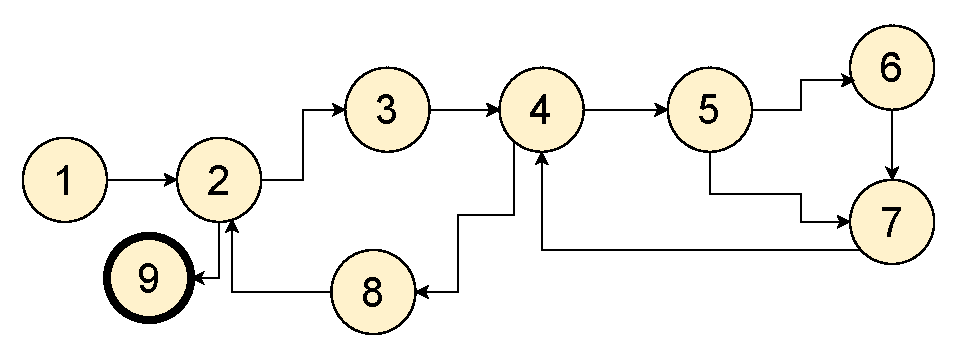
\includegraphics[width=0.8\textwidth]{hw1/q4_graph.pdf}

\begin{parts}
	\part[8] Provide a simple example using C source code that generates the control-flow graph considered.
	The code should be a valid C code fragment. Do not add ``include'' preprocessor directives or a ``main'' function. Do not use gotos unless necessary. Label the source code statements using comments with the CFG node names.
    \pf{I'm not sure that the solution is correct in terms of naming. The statement 2 has to have three parts: the init (2a), the condition (2b), and the increment (2c). Statement 2a is part of the same basic block as statement 1, so CFG 1 is fine. The same happens between 8 and 2c. So the line with the for loop should have the comment: // 1, 2, 8. You can also delete the current lines with comments 1 and 8. I could be missing something so double check again.}
    \answerspace{10}
    \answer{
        \verbatiminput{hw1/q4_answer.c}
    }


	\part[3] List the testing requirement set necessary to satisfy node coverage.
    \answerspace{10}
    \answer{
    TR = \{1, 2, 3, 4, 5, 6, 7, 8, 9\}
    }

    \part[4] List the testing requirement set necessary to satisfy edge coverage.
    \answerspace{10}
    \answer{
    TR=\{[1,2],[2,3],[2,9],[3,4],[4,5],[4,8],[5,6],[5,7],[6,7],[7,4],[8,2]\}
    }

	\part[2] List all the test paths with length up to 7, inclusive. Each path should be listed on its own line.
    \answerspace{10}
    
    \answer{
    [1,2,3,4,8,2,9]
    
    [1,2,9]
    }

\end{parts}

\newpage

\question Please consider the following CFG. \\
% 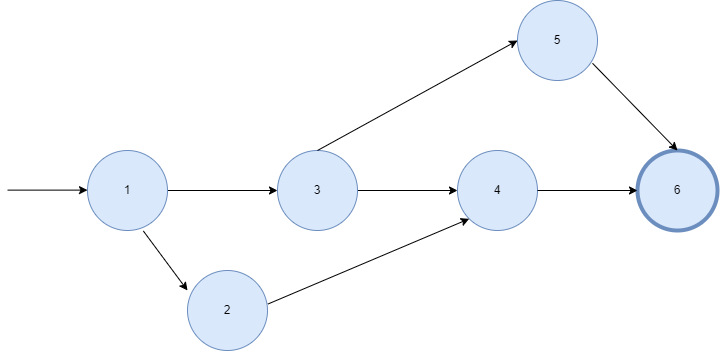
\includegraphics[width=0.6\linewidth]{hw1/cfg2.drawio.png}
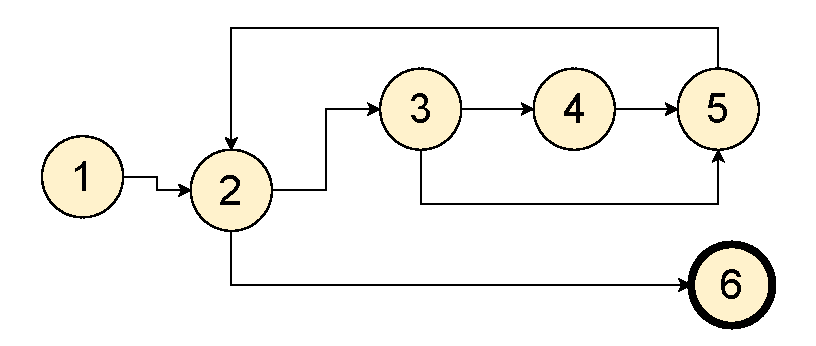
\includegraphics[width=0.8\linewidth]{hw1/q5_graph.pdf}

\begin{parts}

	\part[8] Provide a simple example using C source code that generates the control-flow graph considered.
	The code should be a valid C code fragment. Do not add ``include'' preprocessor directives or a ``main'' function. Do not use gotos unless necessary. Label the source code statements using comments with the CFG node names.
    
    \answerspace{10}
    \answer{
        \verbatiminput{hw1/q5_answer.c}
    }
    
	\part[3] List the testing requirement set necessary to satisfy node coverage.
    \answerspace{10}
    \answer{
        TR=\{1,2,3,4,5,6\}
    }
    \part[3] List the testing requirement set necessary to satisfy edge coverage.
    \answerspace{10}
    \answer{
    TR=\{[1,2], [2,3], [2,6], [3,4], [3,5], [4,5], [5,2]\}
    }
    \part[3] List all the test paths with length less than or equal to 5, inclusive. Each path should be listed on its own line.
    \answerspace{10} 
    \answer{
        [1,2,6]
        [1,2,3,5,2,6]
    }
\end{parts}

\if 0 %%%%%%%%%%%%%%%%%%%%%%%%%%%%%%%%%%%%%%%%%
	\question[10]
	\answerspace{30}
	\answer{}

	\question
	\begin{parts}
		\part[6]
		\answerspace{20}
		\answer{}

		\part[2]
		\answerspace{10}
		\answer{}

	\end{parts}
\fi %%%%%%%%%%%%%%%%%%%%%%%%%%%%%%%%%%%%%%%%%

	\newpage
	\begin{center}
		[EMPTY PAGE]
	\end{center}

\end{questions}

\end{document}
